\documentclass[tikz,border=10pt]{standalone}
\usepackage{tikz}
\usetikzlibrary{arrows.meta, positioning, fadings, shapes.arrows}

\begin{document}
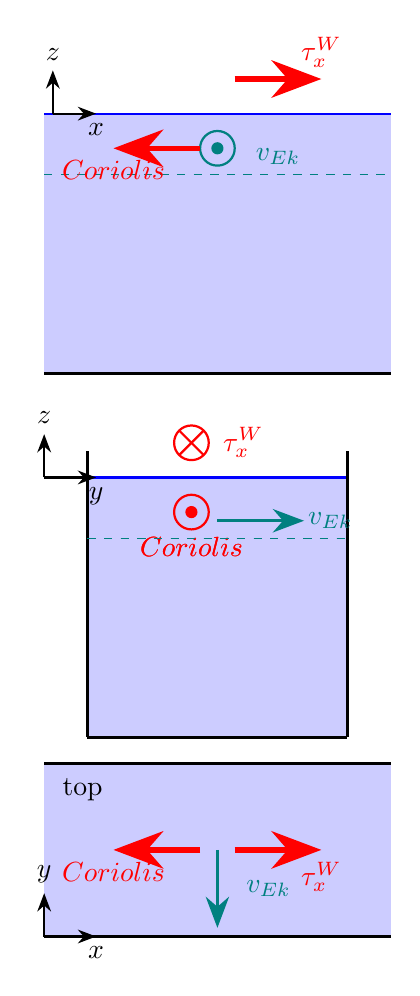
\begin{tikzpicture}[scale=1.1, >=Stealth]

% draw a sea surface height $\eta$ that tilts up to the right:

%draw a dashed line at (-0.5, 0 to 3.5, 0) to represent the sea surface at rest
\fill[blue!20] (-0.5,-3) rectangle (3.5,0);
\draw[thick, blue] (-0.5,0) -- (3.5,0.0) node[midway, above]{};
\draw[very thick, black] (-0.5,-3) -- (3.5,-3) node[midway, above]{};


%Draw a circle in the middle of the line at x=1.5 z=-0.3 that has an X through it to look like the back of an arrowhead
\draw[thick, teal] (1.5,-0.4) circle (0.2);
% draw a dot in the center of circle:
\fill[teal] (1.5,-0.4) circle (2pt);
\draw[dashed, teal] (-0.5,-0.7) -- (3.5,-0.7) node[midway, above]{};
% label it with $v_{Ek}$
\node[text=teal] at (2.2,-0.5) {$v_{Ek}$};

% draw a horizontal arrow to right of circle with label $fv_g$
\draw[thick, red, -{Stealth[scale=1.5]}, line width=2pt] (1.7,0.4) -- (2.7,0.4) node[right, above] {$\tau^W_{x}$};
\draw[thick, red, -{Stealth[scale=1.5]}, line width=2pt] (1.3,-0.4) -- (0.3,-0.4) node[right, below] {$Coriolis$};

% small axes indicating x and z directions:
\draw[->, thick] (-0.4,0) -- (0.1,0) node[below] {$x$};
\draw[->, thick] (-0.4,0) -- (-0.4,0.5) node[above] {$z$};

% make another part of the figure below the part above:
\begin{scope}[yshift=-4.2cm]

    % draw three vertical lines representing the sea surface heihght

    \fill[blue!20] (0,-3) rectangle (3,0);
    \draw[thick, blue] (0,0) -- (3,0.0) node[midway, above]{};
    \draw[very thick, black] (0,-3) -- (3,-3) node[midway, above]{};
    \draw[very thick, black] (0,0.3) -- (0,-3) node[midway, above]{};
    \draw[very thick, black] (3,0.3) -- (3,-3) node[midway, above]{};
    % add a hatched region beneath this to indicate sea floor better:
    \draw[dashed, teal] (0,-0.7) -- (3,-0.7) node[midway, above]{};
    % thick teal arrow pointing down from the middle of the line at x=1.5 z=-0.3
    \draw[thick, teal, -{Stealth[scale=1.5]}, line width=1pt] (1.5,-0.5) -- (2.5,-0.5) node[midway, right] {$\ \ \ \ v_{Ek}$};

    % draw a red circle at (1.2,-0.4) with a dot in the center, labeled "Coriolis":
    \draw[thick, red] (1.2,-0.4) circle (0.2);
    % draw a dot in the center of circle:
    \fill[red] (1.2,-0.4) circle (2pt);
    % label it with "Coriolis"
    \node[text=red] at (1.2,-0.8) {$Coriolis$};

    % draw a red circle at (1.2,-0.4) with a dot in the center, labeled "Coriolis":
    \draw[thick, red] (1.2,0.4) circle (0.2);
    % draw an x in this circle with the same size as the radius of the circle:
    \draw[thick, red] (1.2,0.4) -- (1.2+0.141,0.4+.141);
    \draw[thick, red] (1.2,0.4) -- (1.2-0.141,0.4+0.141);
    \draw[thick, red] (1.2,0.4) -- (1.2+0.141,0.4-0.141);
    \draw[thick, red] (1.2,0.4) -- (1.2-0.141,0.4-0.141);
    % label as wind stress:
    \node[text=red] at (1.8,0.4) {$\tau^W_{x}$};

    % label it with "Coriolis"
    \node[text=red] at (1.2,-0.8) {$Coriolis$};

    \draw[dashed, teal] (0,-0.7) -- (3,-0.7) node[midway, above]{};


    % now draw the same thing from above:
    % small axes indicating x and y directions:
    \draw[->, thick] (-0.5,0) -- (0.1,0) node[below] {$y$};
    \draw[->, thick] (-0.5,0) -- (-0.5,0.5) node[above] {$z$};

\end{scope}

% make another part of the figure below the part above:
\begin{scope}[yshift=-9.5cm]


    % draw three vertical lines representing the sea surface heihght

    \fill[blue!20] (-0.5,0) rectangle (3.5,2);
    \draw[very thick, black] (-0.5,0) -- (3.5,0) node[midway, above]{};
    \draw[very thick, black] (-0.5,2) -- (3.5,2) node[midway, above]{};
    % add a hatched region beneath this to indicate sea floor better:

    % draw a horizontal arrow to right of circle with label $fv_g$

    \draw[thick, red, -{Stealth[scale=1.5]}, line width=2pt] (1.7,1) -- (2.7,1) node[right, below] {$\tau^W_{x}$};
    \draw[thick, red, -{Stealth[scale=1.5]}, line width=2pt] (1.3,1) -- (0.3,1) node[left, below] {$Coriolis$};

    % thick teal arrow pointing down from the middle of the line at x=1.5 z=-0.3
    \draw[thick, teal, -{Stealth[scale=1.5]}, line width=1pt] (1.5,1) -- (1.5,0.1) node[midway, right] {$\ \ v_{Ek}$};

    % now draw the same thing from above:
    % small axes indicating x and y directions:
    \draw[->, thick] (-0.5,0) -- (0.1,0) node[below] {$x$};
    \draw[->, thick] (-0.5,0) -- (-0.5,0.5) node[above] {$y$};
    \node at (-0.4, 1.7) [below, right] {top};

\end{scope}

\end{tikzpicture}
\end{document}
